% -*- TeX-master: "Qualificacao.tex" -*-
%!TEX root = Qualificacao.tex
\chapter{Virtual Reference Feedback Tuning}\label{cap:VRFT}
\vspace{-1cm}

% \section{Introdução}\label{sec:introvrft}

% O método \emph{Virtual Reference Feedback Tunning}, ou simplesmente VRFT, é um procedimento que visa o projeto de controladores realimentados a partir somente de dados amostrados do processo, sem a necessidade de um modelo que descreva este último. Com isso, se classifica como um método de controle baseado em dados, ou DDC.

The \textit{Virtual Reference Feedback Tunning} method, or simply VRFT, proposed by \cite{campi2002}, is a procedure that aims to design closed loop controllers based only on data sampled from the process, without the need for a model that describes that process itself. Thus, it is classified as a data-based control method, or DDC.

% O principal objetivo deste método é ajustar os parâmetros de um controlador, definido por uma função paramétrica, a partir de dados amostrados do processo, a fim de que o sinal de saída do processo controlado tenha um comportamento o mais próximo possível do sinal de saída de um modelo de referência previamente definido.
The main objective of this method is to adjust the parameters of a controller, defined by a parametric function like \eqref{eq:uknl_par}, using the process sampled data only, so that the output signal of the controlled process, $y_\theta(k)$ behaves as close as possible to the output signal $\tilde{y}$ of a previously defined reference model as defined in \eqref{eq:Mmap}.
To reach this objective, VRFT aims to optimize the tracking error by minimizing a performance index $J_y(\vtheta)$ as stated in \eqref{eq:Jy}, rewritten here for convenience:
\begin{equation}
   J^N_y(\bm{\theta}) \triangleq \lim_{N \to \infty}  \frac{1}{N} \sum_{k=1}^N \left[y(k,\vtheta) - \hat{y}(k)\right]^2 = 
    \left\lVert y_\theta - \tilde{y} \right\lVert^{2}
   \label{eq:Jy},
\end{equation}
% sendo $N$ o número de dados amostrados,  $\vtheta = \begin{bmatrix} \theta_1 & \theta_2 & \cdots & \theta_N \end{bmatrix}^T \in \R^n$ um vetor de parâmetros, $k$ um índice temporal
% % , $\E[\cdot]$ um operador que representa o cálculo da esperança
% com $y_r(k,\vtheta)$ e $y_{MR}(k)$, definidos como se segue:
where $N$ represents the number of data samples, $\vtheta = \begin{bmatrix} \theta_1 & \theta_2 & \cdots & \theta_N \end{bmatrix}^T \in \R^N$ a vector of parameters and $k$ a temporal index. The signal $y_\theta(k) \in \R $ represents the output of the  system controlled with the parametrized controller $C_\theta$, and $\tilde{y}(k) \in \mathbb{R}$ are the output of a reference model $M$, both subject to the same reference signal.

% \begin{itemize}
   % % \item $y_r(k,\vtheta)$ representa a resposta obtida em malha fechada utilizando um controlador com parâmetros $\vtheta$, quando sobre o efeito de um sinal de referência $r(k)$, ou seja
   % \item $y_{r}(k)$ represents the response obtained in closed loop using a controller with  parameters $\vtheta$, when under the effect of a  reference signal $r(k)$, i.e.
      % \begin{equation}
         % y_r(k,\vtheta) \triangleq M(q,\vtheta)r(k)
         % \label{eq:yr},
      % \end{equation}
      % % onde $M(q,\vtheta)$ representa o modelo em malha fechada do sistema controlado, função do vetor de parâmetros $\vtheta$ e $q$ um operador de deslocamento temporal.
      % where $M(q,\vtheta)$ represents the closed loop model of the controlled system, function of the vector of parameters, $\vtheta$, and a time displacement operator, $q$.
      % % \item $y_{mr}(k)$ representa a resposta temporal obtida ao se aplicar o sinal de referência $r(k)$ como sinal de entrada de um modelo $M(q)$, conhecido como \textit{modelo de referência} e que representa o comportamento desejado em malha fechada, ou seja
   % \item $y_{MR}(k)$ represents the temporal response obtained by applying the reference signal $r(k)$ as an input signal for a model $M(q)$, known as a \textit{reference model} and representing the desired closed-loop behavior, i.e.
      % \begin{equation}
         % y_{MR}(k) \triangleq M(q)r(k)
         % \label{eq:yMR},
      % \end{equation}
% \end{itemize}

% Para alcançar o objetivo de minimizar \eqref{eq:Jy}, \cite{campi2002}, para o caso linear, e \cite{campi2006}, para o caso não linear, mostram que, sob certas condições, apresentadas na sequência, ao se minimizar um índice de custo definido como
To achieve the objective of minimizing \eqref{eq:Jy}, \cite{campi2002}, for the linear case, and \cite{campi2006}, for the non-linear case, show that, under certain conditions, presented in sequence, when minimizing a cost index defined as
\begin{equation}
   J_{VR}(\vtheta) \triangleq \lim_{N \to \infty}  \frac{1}{N} \sum_{k=1}^N \left[u(k) - C_\theta(q,\vtheta)\bar{e}(k)\right]^2
   \label{eq:Jvr},
\end{equation}
% minimiza-se também o índice $J_y(\theta)$ definido em ~\eqref{eq:Jy}. Em \eqref{eq:Jvr}, $u(k)$ representa o sinal de entrada aplicado ao processo durante a coleta de dados, $C(q,\vtheta)$ o modelo do controlador a ser ajustado e $e(k)$ é o chamado \textit{erro virtual}, definido como
the index $J_y(\vtheta)$ defined in~\eqref{eq:Jy} is also minimized. In~\eqref{eq:Jvr}, $u(k)$ represents the input signal applied to the process during data collection, $C (q,\vtheta)$ the controller model to be adjusted and $\bar{e}(k)$ is the so-called \textit{virtual error}, defined as
\begin{equation}
   \ev(k) = \rv(k) - y(k) 
   \label{eq:ev},
\end{equation}
% onde $\rv$ é o sinal de \textit{referência virtual}, obtido ao se filtrar a saída $y(k)$ pelo modelo de referência inverso, na forma
where $\rv$ is a signal called \textit{virtual reference}, obtained by filtering the output $y(k)$ by the inverse reference model $M^{-1}(q)$, in the form
\begin{equation}
   \rv(k) = M^{-1}(q)y(k)
   \label{eq:refvirt}.
\end{equation}

% O termo ``virtual'' é adotado nos sinais de referência e erro para enfatizar que nenhum destes sinais são fisicamente disponíveis, mas apenas calculados para fins de projeto do controlador. \todo{melhorar isso aqui.}
The term ``virtual'' is adopted in reference tracking error signals to emphasize that none of these signals are physically available, but only calculated for controller design purposes, as will be better explained latter. \todo{improve this here.}

% Como mencionado anteriormente, para que $J_y(\vtheta)$ e  $J_{VR}(\vtheta)$ apresentem seus valores mínimos para a mesma solução de parâmetros $\vtheta$, certas condições devem ser satisfeitas. Estas condições são apresentadas na sequência, logo após algumas definições que se mostram importantes para o restante do capítulo.
The condition for  $J_y(\vtheta)$ and $J_{VR}(\vtheta)$ reach their minimum values for the same parameter solution $\vtheta$ are presented in sequence, right after some definitions that are important for the rest of the chapter.

\section{Basic definitions}\label{sec:vrft_basic_def}

\begin{defn}[Ideal Controller]\label{def:idealControler}
   \todo[inline]{Put definition here.}
\end{defn}

\begin{assum}[Noise free]\label{ass:noiseFree} 
   The system is not affected by noise.
\end{assum}

\begin{assum}[Matched control]\label{ass:machedControl} %% Assumption By of \citep{bazanella2012} pg 13 
   The ideal controller belongs to control model class considered, i.e. $C_0(q) \in \mathscr{C}$, or, equivalently
   \begin{equation}
      \exists \bm{\theta}_0 : C(q,\bm{\theta}_0)=C_0(q)
      \label{eq:assumpMatched}.
   \end{equation}
\end{assum}

\begin{figure}[H]
   \centering
   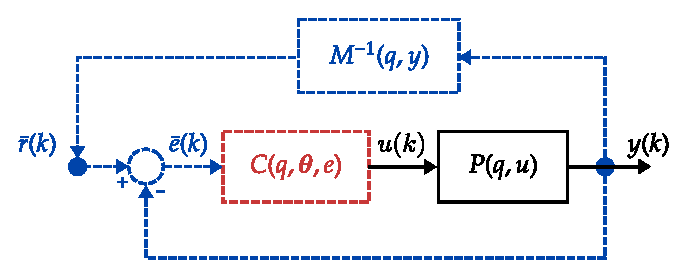
\includegraphics{Figs/diagrama_VRFT.eps}
   \caption{ Experiment to obtain the data used to identify the controller parameters by the VRFT method:
   real data (\textit{black solid lines}), virtual data (\textit{blue dashed lines}) and the cotroller to tune in (\textit{red dashed block}).}
   \label{fig:Figs-diagrama_VRFT-eps}
\end{figure}

\section{Filtro Caso não Linear}%
\label{sec:filtro_caso_não_linear}

Objetivo do filtro
\begin{equation}
   J_{\mathrm{VRFT}}\left(\theta^{+}\right):=\left\|F\left[C_{\theta}+[\tilde{e}]\right]-F[\tilde{u}]\right\|^{2}
   \label{eq:JVR}
\end{equation}
Deseja-se selecionar um filtro tal que \begin{equation}
   \left.\frac{\partial^{2} J_{\mathrm{VRFT}}\left(\theta^{+}\right)}{\partial \theta^{+2}}\right|_{\theta_{0}^{+}}=\left.\frac{\partial^{2} J\left(\theta^{+}\right)}{\partial \theta^{+2}}\right|_{\theta_{0}^{+}}
   \label{eq:condToF}
\end{equation}

\begin{theorem}
   Se 
   \begin{equation}
       F=(I-M D)\left(\left.\frac{\partial P[u]}{\partial u}\right|_{\tilde{u}}\right)
       \label{eq:FiltroVRFTNL}
   \end{equation}
   então \eqref{eq:condToF} é satisfeita.
\end{theorem}


\section{Prova da escolha do filtro VRFT}%
\label{sec:prova_da_escolha_do_filtro_vrft}
Note que
\begin{equation}
\tilde{u}=C_{\theta_{0}^{+}}[\tilde{e}]
\label{eq:uTil}
\end{equation}
uma vez que
\begin{align}
   \tilde{u}&=P^{-1}[\hat{y}]=P^{-1}\left[(I-M D)^{-1}(I-M D) \hat{y}\right] \nonumber\\
            &= P^{-1}\left[(I-M D)^{-1}(M \tilde{r}-M D \tilde{y})\right]=P^{-1}\left[(I-M D)^{-1} M \tilde{e}\right] = C^{0}[\tilde{e}] \nonumber\\
            &=C_{\theta_{0}^{+}}[\tilde{e}].
\end{align}

De forma semelhante
\begin{equation}
   \tilde{y}=y_{\theta_{0}^{+}}
\label{eq:yqp}
\end{equation}
uma vez que, $\tilde{y}=P[\tilde{u}]$ a partir de \eqref{eq:uTil}, assumindo $\tilde{e}=\tilde{r}-D \tilde{y}$,  tem-se que $\tilde{y}=P\left[C_{\theta_{0}^{+}}[\tilde{e}]\right]=$$P\left[C_{\theta_{0}^{+}}[\tilde{r}-D \tilde{y}]\right]$. Como
$y_{\theta_{0}^{+}}=P\left[C_{\theta_{0}^{+}}\left[\tilde{\tilde{r}}-D y_{\theta_{0}^{+}}\right]\right]$, 
$\tilde{y}$ e $y_{\theta_{0}^{+}}$ corresponde ao mesmo $\tilde{r}$ no mapa $r \mapsto y$ dado por $y=P\left[C_{\theta_{0}^{+}}[r-D y]\right]$.
% $\tilde{y}$ e $y_{\theta_{0}^{+}}$ corresponde ao mesmo $\tilde{r}$ in the $r$ to $y$ map given by $y=P\left[C_{\theta_{0}^{+}}[r-D y]\right]$
Uma vez que tal mapa, dado um $r$ há somente um $y$ correspondente, conclui-se \eqref{eq:yqp}.
De \eqref{eq:yqp} é possível concluir que 
\begin{equation}
   \tilde{r}-D y_{\theta_{0}^{+}}=\tilde{e},
\label{eq:eTil}
\end{equation}
que, em \eqref{eq:uTil}, resulta em
\begin{equation}
\tilde{u}=C_{\theta_{0}^{+}}\left[\tilde{r}-D y_{\theta_{0}^{+}}\right].
\label{eq:uTil_2}
\end{equation}

% Parei aqui...

Por simplicidade e maior clareza no desenvolvimento, adota-se a seguinte notação:
\begin{align}
   x_{\theta^{+}} &\triangleq F\left[C_{\theta^{+}}[\tilde{e}]\right]-F[\tilde{u}] \label{eq:x} \\
   w_{\theta^{+}} &\triangleq y_{\theta^{+}}-\tilde{y} \label{eq:w} \\
   \frac{\partial g}{\partial \theta^{+}} &\triangleq 
   \begin{bmatrix} 
      \partial g_1/\partial \theta^{+}_1 & \dots & \partial g_1/\partial \theta^{+}_j & \dots & \partial g_1/\partial \theta^{+}_{n_{\theta +}} \\
      \vdots &  & \vdots & & \vdots \\
      \partial g_i/\partial \theta^{+}_1 & \dots & \partial g_i/\partial \theta^{+}_j & \dots & \partial g_i/\partial \theta^{+}_{n_{\theta +}} \\
      \vdots & & \vdots & & \vdots \\
      \partial g_N/\partial \theta^{+}_1 & \dots & \partial g_N/\partial \theta^{+}_j & \dots & \partial g_N/\partial \theta^{+}_{n_{\theta +}}
   \end{bmatrix} \label{eq:partg}
\end{align}
   % \partial g /\partial \theta^{+} &\triangleq \partial g(i)  /\partial \theta^{+}_j \label{eq:partg}
\todo{Olhar \eqref{eq:partg}. Não é bem isso, na verdade é uma matriz.} 
Sendo \eqref{eq:partg} (em que $g$ é uma função genérica) definida tal que o $(i,j)$-ésimo elemento é $\partial g(i)  /\partial \theta^{+}_j$, de modo que as colunas $(j)$ correspondem às derivadas de $g$ em relação a diferentes parâmetros e as linhas $(i)$ correspondem à evolução temporal.

Usando \eqref{eq:x} e \eqref{eq:w}, as função de custo \eqref{eq:JVR} e \eqref{eq:Jy} são rescritas como
$$
J_{\mathrm{VR}}\left(\theta^{+}\right)=\left\|x_{\theta^{+}}\right\|^{2} \qquad J\left(\theta^{+}\right)=\left\|w_{\theta^{+}}\right\|^{2}
$$
Calculando a primeira e segunda derivadas de $J_{\mathrm{VR}}\left(\theta^{+}\right)$ com respeito ao vetor de parâmetros $\theta^+$, para aproximação por séries de Taylor:
\begin{align}
   \frac{\partial J_{\mathrm{VR}}\left(\theta^{+}\right)}{\partial \theta^{+}} &=\frac{\partial x_{\theta^{+}}^{T} x_{\theta^{+}}}{\partial \theta^{+}} = 2 x_{\theta^{+}}^{T}\left(\frac{\partial x_{\theta^{+}}}{\partial \theta^{+}}\right), \\
\frac{\partial^{2} J_{\mathrm{VR}}\left(\theta^{+}\right)}{\partial \theta^{+2}}&= 2 x_{\theta^{+}}^{T}\left(\frac{\partial^{2} x_{\theta^{+}}}{\partial \theta^{+2}}\right)
+2\left(\frac{\partial x_{\theta^{+}}}{\partial \theta^{+}}\right)^{T}\left(\frac{\partial x_{\theta^{+}}}{\partial \theta^{+}}\right). 
\end{align}
Utilizando \eqref{eq:x} e \eqref{eq:uTil} e calculando as derivadas para o ponto de equilíbrio $\theta^{+}_0$, resulta em
\begin{align}
\left.J_{\mathrm{VR}}\left(\theta^{+}\right)\right|_{\theta_{0}^{+}}
& =\left.\frac{\partial J_{\mathrm{VR}}\left(\theta^{+}\right)}{\partial \theta^{+}}\right|_{\theta_{0}^{+}} =0 \label{eq:JVRTaylor_1}\\
   \left.\frac{\partial^{2} J_{\mathrm{VRFT}}\left(\theta^{+}\right)}{\partial \theta^{+2}}\right|_{\theta_{0}^{+}} &= 2\left(\left.\frac{\partial x_{\theta^{+}}}{\partial \theta^{+}}\right|_{\theta_{0}^{+}}\right)^{T}\left(\left.\frac{\partial x_{\theta^{+}}}{\partial \theta^{+}}\right|_{\theta_{0}^{+}}\right) \label{eq:JVRTaylor_2}
\end{align}

Fazendo o mesmo procedimento para $J\left(\theta^{+}\right)=\left\|w_{\theta^{+}}\right\|^{2}$:
\begin{align}
\frac{\partial J\left(\theta^{+}\right)}{\partial \theta^{+}} 
   &=\frac{\partial w_{\theta^{+}}^{T} w_{\theta^{+}}}{\partial \theta^{+}}=2 w_{\theta^{+}}^{T}\left(\frac{\partial w_{\theta^{+}}}{\partial \theta^{+}}\right), \\
\frac{\partial^{2} J\left(\theta^{+}\right)}{\partial \theta^{+2}}&= 2 x_{\theta^{+}}^{T}\left(\frac{\partial^{2} w_{\theta^{+}}}{\partial \theta^{+2}}\right) 
+2\left(\frac{\partial w_{\theta^{+}}}{\partial \theta^{+}}\right)^{T}\left(\frac{\partial w_{\theta^{+}}}{\partial \theta^{+}}\right).
\label{eq:}
\end{align}
Usando \eqref{eq:w} e \eqref{eq:yqp}:
\begin{align}
\left.J\left(\theta^{+}\right)\right|_{\theta_{0}^{+}}                                                                      
&=\left.\frac{\partial J\left(\theta^{+}\right)}{\partial \theta^{+}}\right|_{\theta_{0}^{+}}=0 \label{eq:JyTaylor_1} \\
   \left.\frac{\partial^{2} J\left(\theta^{+}\right)}{\partial \theta^{+2}}\right|_{\theta_{0}^{+}} &= 2\left(\left.\frac{\partial w_{\theta^{+}}}{\partial \theta^{+}}\right|_{\theta_{0}^{+}}\right)^{T}\left(\left.\frac{\partial w_{\theta^{+}}}{\partial \theta^{+}}\right|_{\theta_{0}^{+}}\right) . \label{eq:JyTaylor_2}
\end{align}

Somando os termos de \eqref{eq:JVRTaylor_1} a \eqref{eq:JVRTaylor_2}, e os \eqref{eq:JyTaylor_1} e \eqref{eq:JyTaylor_2}, tem-se, respectivamente uma aproximação de segunda ordem por séries de Taylor. E para que o objetivo do filtro \eqref{eq:FiltroVRFTNL} seja alcançado, ou seja $ J_{\mathrm{VR}}\left(\theta^{+}\right) \approx J\left(\theta^{+}\right)$, comparando \eqref{eq:JVRTaylor_2} com \eqref{eq:JyTaylor_2}, deve-se ter  
\begin{equation}
   \left.\frac{\partial x_{\theta^{+}}}{\partial \theta^{+}}\right|_{\theta_{0}^{+}}=\left.\frac{\partial w_{\theta^{+}}}{\partial \theta^{+}}\right|_{\theta_{0}^{+}}
   \label{eq:FilterObjective}
\end{equation}

Usando a notação 

\begin{equation}
   \frac{\partial P[u]}{\partial u} \triangleq 
   \begin{bmatrix} 
      \partial P[u]_1/\partial u_0 & \dots & \partial P[u]_1/\partial u_{(j-1)} & \dots & \partial P[u]_1/\partial u_{(N-1)} \\
      \vdots &  & \vdots & & \vdots \\ 
      \partial P[u]_i/\partial u_0 & \dots & \partial P[u]_i/\partial u_{(j-1)} & \dots & \partial P[u]_i/\partial u_{(N-1)} \\
      \vdots & & \vdots & & \vdots \\ 
      \partial P[u]_N/\partial u_0 & \dots & \partial P[u]_N/\partial u_{(j-1)} & \dots & \partial P[u]_N/\partial u_{(N-1)}
   \end{bmatrix}  
   \label{eq:PuDu}
\end{equation}
e resolvendo o lado esquerdo de \eqref{eq:FilterObjective}, considerando que o filtro $F$ é linear, chega-se a
\begin{equation}
   \left.\frac{\partial x_{\theta^{+}}}{\partial \theta^{+}}\right|_{\theta_{0}^{+}}=\left.\frac{\partial F\left[C_{\theta^{+}}[\tilde{e}]\right]}{\partial \theta^{+}}\right|_{\theta_{0}^{+}}=F\left(\left.\frac{\partial C_{\theta^{+}}[\tilde{e}]}{\partial \theta^{+}}\right|_{\theta_{0}^{+}}\right)
\label{eq:28}
\end{equation}

Como $C_{\theta_0^+} = \tilde{u}$, ver \eqref{eq:uTil}, o lado direito de \eqref{eq:FilterObjective} é calculado como
\begin{align}
\left.\left.\frac{\partial P[u]}{\partial u}\right|_{\tilde{u}} \frac{\partial C_{\theta_{0}^{+}}[e]}{\partial e}\right|_{\tilde{e}} &=\left.\frac{\partial P\left[C_{\theta_{0}^{+}}[e]\right]}{\partial e}\right|_{\tilde{e}} \nonumber\\
&=\left.\frac{\partial(I-M D)^{-1} M[e]}{\partial e}\right|_{\tilde{e}} \nonumber\\
&=(I-M D)^{-1} M .
\label{eq:29}
\end{align}

Aplicando a regra da cadeia, em $(\partial y_{\theta_0^+}/\partial \theta^+)$:
\begin{align}
\left.\frac{\partial y_{\theta^{+}}}{\partial \theta^{+}}\right|_{\theta_{0}^{+}}=&\left.\frac{\partial P\left[C_{\theta^{+}}\left[\tilde{r}-D y_{\theta^{+}}\right]\right]}{\partial \theta^{+}}\right|_{\theta_{0}^{+}} \\
=&\left.\frac{\partial P[u]}{\partial u}\right|_{C_{\theta_{0}^{+}}\left[\tilde{r}-D y_{\theta_{0}^{+}}\right]} 
   \left\{\left.\left.\frac{\partial C_{\theta^{+}}\left[\tilde{r}-D y_{\theta_{0}^{+}}\right]}{\partial \theta^{+}}\right|_{\theta_{0}^{+}}{-\left.\frac{\partial C_{\theta_{0}^{+}}[e]}{\partial e}\right|_{\tilde{r}-D y_{\theta_{0}^{+}}}} \frac{\partial D y_{\theta^{+}}}{\partial \theta^{+}}\right|_{\theta_{0}^{+}}\right\}
\end{align}
%
Usando \eqref{eq:eTil} e \eqref{eq:uTil_2},
\begin{equation}
   \left.\frac{\partial y_{\theta^{+}}}{\partial \theta^{+}}\right|_{\theta_{0}^{+}}=\left.\frac{\partial P[u]}{\partial u}\right|_{\tilde{u}}\left\{\left.\frac{\partial C_{\theta^{+}}[\tilde{e}]}{\partial \theta^{+}}\right|_{\theta_{0}^{+}}\right.
   \left.-\left.\left.\frac{\partial C_{\theta_{0}^{+}}[e]}{\partial e}\right|_{\tilde{e}} \frac{\partial D y_{\theta^{+}}}{\partial \theta^{+}}\right|_{\theta_{0}^{+}}\right\}
\end{equation}


e então
\begin{equation}
   \left.\left.\frac{\partial P[u]}{\partial u}\right|_{\tilde{u}} \frac{\partial C_{\theta^{+}}[\tilde{e}]}{\partial \theta^{+}}\right|_{\theta_{0}^{+}}
   =
   \left.\frac{\partial y_{\theta^{+}}}{\partial \theta^{+}}\right|_{\theta_{0}^{+}}+\left.\left.\left.\frac{\partial P[u]}{\partial u}\right|_{\tilde{u}} \frac{\partial C_{\theta_{0}^{+}}[e]}{\partial e}\right|_{\tilde{e}} \frac{\partial D y_{\theta^{+}}}{\partial \theta^{+}}\right|_{\theta_{0}^{+}}.
\end{equation}

Substituindo em \eqref{eq:29} resulta em
\begin{equation}
   \left.\frac{\partial y_{\theta^{+}}}{\partial \theta^{+}}\right|_{\theta_{0}^{+}}+(I-M D)^{-1} M \frac{\partial D y_{\theta^{+}}}{\partial \theta^{+}} \left.\right|_{\theta_{0}^{+}}
   =\left.\left.\frac{\partial P[u]}{\partial u}\right|_{\tilde{u}} \frac{\partial C_{\theta^{+}}[\tilde{e}]}{\partial \theta^{+}}\right|_{\theta_{0}^{+}},
\end{equation}
que, multiplicando por $(I-MD)$, nos dá
\begin{equation}
   \left.\frac{\partial y_{\theta^{+}}}{\partial \theta^{+}}\right|_{\theta_{0}^{+}}-\left.M D \frac{\partial y_{\theta^{+}}}{\partial \theta^{+}}\right|_{\theta_{0}^{+}}+\left.M \frac{\partial D y_{\theta^{+}}}{\partial \theta^{+}}\right|_{\theta_{0}^{+}}
   =\left.\left.(I-M D) \frac{\partial P[u]}{\partial u}\right|_{\tilde{u}} \frac{\partial C_{\theta^{+}}[\tilde{e}]}{\partial \theta^{+}}\right|_{\theta_{0}^{+}}
\end{equation}
Por fim, o termo do lado direito de \eqref{eq:FilterObjective}, pode ser escrito como
\begin{equation}
   \left.\frac{\partial w_{\theta^{+}}}{\partial \theta^{+}}\right|_{\theta_{0}^{+}} =\left.\frac{\partial y_{\theta^{+}}}{\partial \theta^{+}}\right|_{\theta_{0}^{+}} 
   =\left.\left.(I-M D) \frac{\partial P[u]}{\partial u}\right|_{\tilde{u}} \frac{\partial C_{\theta^{+}}[\tilde{e}]}{\partial \theta^{+}}\right|_{\theta_{0}^{+}}
\end{equation}
que, comparando com \eqref{eq:28}, conclui-se que
\begin{equation}
   F=(I-M D)\left(\left.\frac{\partial P[u]}{\partial u}\right|_{\tilde{u}}\right) .
\label{eq:FiltroFinal}
\end{equation}


